% Created by tikzDevice version 0.7.0 on 2014-02-02 01:44:57
% !TEX encoding = UTF-8 Unicode
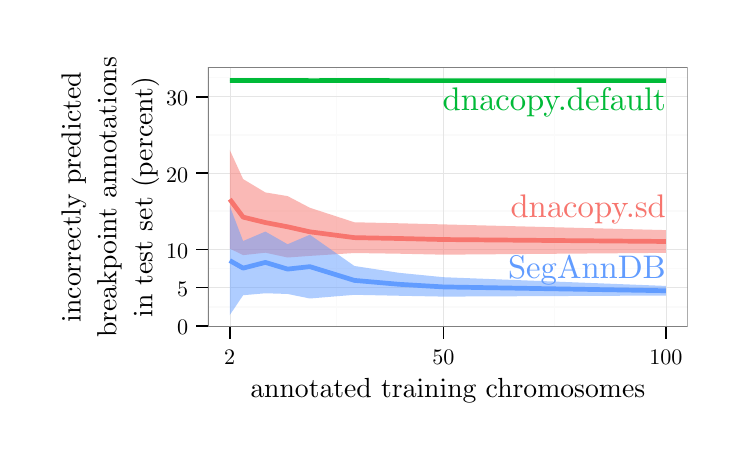
\begin{tikzpicture}[x=1pt,y=1pt]
\definecolor[named]{fillColor}{rgb}{1.00,1.00,1.00}
\path[use as bounding box,fill=fillColor,fill opacity=0.00] (0,0) rectangle (252.94,144.54);
\begin{scope}
\path[clip] (  0.00,  0.00) rectangle (252.94,144.54);
\definecolor[named]{drawColor}{rgb}{1.00,1.00,1.00}
\definecolor[named]{fillColor}{rgb}{1.00,1.00,1.00}

\path[draw=drawColor,line width= 0.6pt,line join=round,line cap=round,fill=fillColor] (  0.00,  0.00) rectangle (252.94,144.54);
\end{scope}
\begin{scope}
\path[clip] ( 65.15, 36.44) rectangle (238.49,130.09);
\definecolor[named]{fillColor}{rgb}{1.00,1.00,1.00}

\path[fill=fillColor] ( 65.15, 36.44) rectangle (238.49,130.09);
\definecolor[named]{drawColor}{rgb}{0.98,0.98,0.98}

\path[draw=drawColor,line width= 0.6pt,line join=round] ( 65.15, 43.70) --
	(238.49, 43.70);

\path[draw=drawColor,line width= 0.6pt,line join=round] ( 65.15, 57.50) --
	(238.49, 57.50);

\path[draw=drawColor,line width= 0.6pt,line join=round] ( 65.15, 78.19) --
	(238.49, 78.19);

\path[draw=drawColor,line width= 0.6pt,line join=round] ( 65.15,105.79) --
	(238.49,105.79);

\path[draw=drawColor,line width= 0.6pt,line join=round] ( 65.15,126.49) --
	(238.49,126.49);

\path[draw=drawColor,line width= 0.6pt,line join=round] (111.62, 36.44) --
	(111.62,130.09);

\path[draw=drawColor,line width= 0.6pt,line join=round] (190.41, 36.44) --
	(190.41,130.09);
\definecolor[named]{drawColor}{rgb}{0.90,0.90,0.90}

\path[draw=drawColor,line width= 0.2pt,line join=round] ( 65.15, 36.80) --
	(238.49, 36.80);

\path[draw=drawColor,line width= 0.2pt,line join=round] ( 65.15, 50.60) --
	(238.49, 50.60);

\path[draw=drawColor,line width= 0.2pt,line join=round] ( 65.15, 64.40) --
	(238.49, 64.40);

\path[draw=drawColor,line width= 0.2pt,line join=round] ( 65.15, 91.99) --
	(238.49, 91.99);

\path[draw=drawColor,line width= 0.2pt,line join=round] ( 65.15,119.59) --
	(238.49,119.59);

\path[draw=drawColor,line width= 0.2pt,line join=round] ( 73.03, 36.44) --
	( 73.03,130.09);

\path[draw=drawColor,line width= 0.2pt,line join=round] (150.21, 36.44) --
	(150.21,130.09);

\path[draw=drawColor,line width= 0.2pt,line join=round] (230.61, 36.44) --
	(230.61,130.09);
\definecolor[named]{drawColor}{rgb}{0.97,0.46,0.43}

\path[draw=drawColor,line width= 1.7pt,line join=round] ( 73.03, 82.53) --
	( 77.85, 76.08) --
	( 85.89, 74.12) --
	( 93.93, 72.58) --
	(101.97, 70.77) --
	(118.05, 68.67) --
	(134.13, 68.36) --
	(150.21, 67.98) --
	(230.61, 67.28);
\definecolor[named]{drawColor}{rgb}{0.00,0.73,0.22}

\path[draw=drawColor,line width= 1.7pt,line join=round] ( 73.03,125.46) --
	( 77.85,125.46) --
	( 85.89,125.45) --
	( 93.93,125.44) --
	(101.97,125.41) --
	(118.05,125.42) --
	(134.13,125.41) --
	(150.21,125.40) --
	(230.61,125.40);
\definecolor[named]{drawColor}{rgb}{0.38,0.61,1.00}

\path[draw=drawColor,line width= 1.7pt,line join=round] ( 73.03, 60.38) --
	( 77.85, 57.65) --
	( 85.89, 59.72) --
	( 93.93, 57.30) --
	(101.97, 58.19) --
	(118.05, 53.22) --
	(134.13, 51.81) --
	(150.21, 50.86) --
	(230.61, 49.48);
\definecolor[named]{fillColor}{rgb}{0.97,0.46,0.43}

\path[fill=fillColor,fill opacity=0.50] ( 73.03,100.34) --
	( 77.85, 89.82) --
	( 85.89, 85.00) --
	( 93.93, 83.67) --
	(101.97, 79.46) --
	(118.05, 74.22) --
	(134.13, 73.86) --
	(150.21, 73.45) --
	(230.61, 71.39) --
	(230.61, 63.17) --
	(150.21, 62.51) --
	(134.13, 62.86) --
	(118.05, 63.11) --
	(101.97, 62.07) --
	( 93.93, 61.49) --
	( 85.89, 63.23) --
	( 77.85, 62.34) --
	( 73.03, 64.73) --
	cycle;
\definecolor[named]{fillColor}{rgb}{0.00,0.73,0.22}

\path[fill=fillColor,fill opacity=0.50] ( 73.03,125.51) --
	( 77.85,125.55) --
	( 85.89,125.58) --
	( 93.93,125.60) --
	(101.97,125.58) --
	(118.05,125.64) --
	(134.13,125.67) --
	(150.21,125.70) --
	(230.61,125.83) --
	(230.61,124.96) --
	(150.21,125.10) --
	(134.13,125.15) --
	(118.05,125.20) --
	(101.97,125.25) --
	( 93.93,125.28) --
	( 85.89,125.31) --
	( 77.85,125.37) --
	( 73.03,125.41) --
	cycle;
\definecolor[named]{fillColor}{rgb}{0.38,0.61,1.00}

\path[fill=fillColor,fill opacity=0.50] ( 73.03, 80.06) --
	( 77.85, 67.44) --
	( 85.89, 70.86) --
	( 93.93, 66.28) --
	(101.97, 69.71) --
	(118.05, 58.43) --
	(134.13, 55.96) --
	(150.21, 54.37) --
	(230.61, 51.22) --
	(230.61, 47.75) --
	(150.21, 47.36) --
	(134.13, 47.67) --
	(118.05, 48.01) --
	(101.97, 46.68) --
	( 93.93, 48.32) --
	( 85.89, 48.57) --
	( 77.85, 47.86) --
	( 73.03, 40.70) --
	cycle;
\definecolor[named]{drawColor}{rgb}{0.00,0.73,0.22}

\node[text=drawColor,anchor=base east,inner sep=0pt, outer sep=0pt, scale=  1.18] at (230.61,114.71) {dnacopy.default};
\definecolor[named]{drawColor}{rgb}{0.97,0.46,0.43}

\node[text=drawColor,anchor=base east,inner sep=0pt, outer sep=0pt, scale=  1.18] at (230.61, 76.07) {dnacopy.sd};
\definecolor[named]{drawColor}{rgb}{0.38,0.61,1.00}

\node[text=drawColor,anchor=base east,inner sep=0pt, outer sep=0pt, scale=  1.18] at (230.61, 54.00) {SegAnnDB};
\definecolor[named]{drawColor}{rgb}{0.50,0.50,0.50}

\path[draw=drawColor,line width= 0.6pt,line join=round,line cap=round] ( 65.15, 36.44) rectangle (238.49,130.09);
\end{scope}
\begin{scope}
\path[clip] (  0.00,  0.00) rectangle (252.94,144.54);
\definecolor[named]{drawColor}{rgb}{0.00,0.00,0.00}

\node[text=drawColor,anchor=base east,inner sep=0pt, outer sep=0pt, scale=  0.80] at ( 58.04, 33.50) {0};

\node[text=drawColor,anchor=base east,inner sep=0pt, outer sep=0pt, scale=  0.80] at ( 58.04, 47.29) {5};

\node[text=drawColor,anchor=base east,inner sep=0pt, outer sep=0pt, scale=  0.80] at ( 58.04, 61.09) {10};

\node[text=drawColor,anchor=base east,inner sep=0pt, outer sep=0pt, scale=  0.80] at ( 58.04, 88.69) {20};

\node[text=drawColor,anchor=base east,inner sep=0pt, outer sep=0pt, scale=  0.80] at ( 58.04,116.28) {30};
\end{scope}
\begin{scope}
\path[clip] (  0.00,  0.00) rectangle (252.94,144.54);
\definecolor[named]{drawColor}{rgb}{0.00,0.00,0.00}

\path[draw=drawColor,line width= 0.6pt,line join=round] ( 60.88, 36.80) --
	( 65.15, 36.80);

\path[draw=drawColor,line width= 0.6pt,line join=round] ( 60.88, 50.60) --
	( 65.15, 50.60);

\path[draw=drawColor,line width= 0.6pt,line join=round] ( 60.88, 64.40) --
	( 65.15, 64.40);

\path[draw=drawColor,line width= 0.6pt,line join=round] ( 60.88, 91.99) --
	( 65.15, 91.99);

\path[draw=drawColor,line width= 0.6pt,line join=round] ( 60.88,119.59) --
	( 65.15,119.59);
\end{scope}
\begin{scope}
\path[clip] (  0.00,  0.00) rectangle (252.94,144.54);
\definecolor[named]{drawColor}{rgb}{0.00,0.00,0.00}

\path[draw=drawColor,line width= 0.6pt,line join=round] ( 73.03, 32.18) --
	( 73.03, 36.44);

\path[draw=drawColor,line width= 0.6pt,line join=round] (150.21, 32.18) --
	(150.21, 36.44);

\path[draw=drawColor,line width= 0.6pt,line join=round] (230.61, 32.18) --
	(230.61, 36.44);
\end{scope}
\begin{scope}
\path[clip] (  0.00,  0.00) rectangle (252.94,144.54);
\definecolor[named]{drawColor}{rgb}{0.00,0.00,0.00}

\node[text=drawColor,anchor=base,inner sep=0pt, outer sep=0pt, scale=  0.80] at ( 73.03, 22.72) {2};

\node[text=drawColor,anchor=base,inner sep=0pt, outer sep=0pt, scale=  0.80] at (150.21, 22.72) {50};

\node[text=drawColor,anchor=base,inner sep=0pt, outer sep=0pt, scale=  0.80] at (230.61, 22.72) {100};
\end{scope}
\begin{scope}
\path[clip] (  0.00,  0.00) rectangle (252.94,144.54);
\definecolor[named]{drawColor}{rgb}{0.00,0.00,0.00}

\node[text=drawColor,anchor=base,inner sep=0pt, outer sep=0pt, scale=  1.00] at (151.82, 10.84) {annotated training chromosomes};
\end{scope}
\begin{scope}
\path[clip] (  0.00,  0.00) rectangle (252.94,144.54);
\definecolor[named]{drawColor}{rgb}{0.00,0.00,0.00}

\node[text=drawColor,rotate= 90.00,anchor=base,inner sep=0pt, outer sep=0pt, scale=  1.00] at ( 19.11, 83.26) {incorrectly predicted};

\node[text=drawColor,rotate= 90.00,anchor=base,inner sep=0pt, outer sep=0pt, scale=  1.00] at ( 32.07, 83.26) {breakpoint annotations};

\node[text=drawColor,rotate= 90.00,anchor=base,inner sep=0pt, outer sep=0pt, scale=  1.00] at ( 45.03, 83.26) {in test set (percent)};
\end{scope}
\end{tikzpicture}
